\documentclass[12pt, a4paper, oneside, openright, headinclude, footinclude, BCOR5mm, cleardoublepage=empty,dottedtoc]{scrbook}       

% ********************************************************************
% Packages da utilizzare
%******************************************************* 

	% encoding ad 8 bit per fonts
	\usepackage[T1]{fontenc}

	% inserimento diretto lettere accentate
	\usepackage[utf8]{inputenc}

	% cambia il reset del contatore delle note
	\usepackage{chngcntr}

	% no reset numero del footnote ad ogni capitolo
	\counterwithout{footnote}{chapter}

	% miglioramenti per inserimento figure e tabelle
	\usepackage{float}
	
	% disegno directory tree
	\usepackage{dirtree}

	% lingua principale del documento e sillabazione
	\usepackage[italian]{babel}

	% lingua bibliografia corrispondente a quella del documento
	\usepackage{babelbib}

	% gestione colori (dvipsnames evita problemi se usato con pdfpages, table per righe colori alternati tabelle)
	\usepackage[dvipsnames,table]{xcolor}

	% inserimento documenti pdf
	\usepackage{pdfpages}

	% layout itemize, enumerate e descrizioni
	\usepackage{enumitem}

	% gestione footnote
	\usepackage{footnote}

	% supporto esteso per grafica
	\usepackage{graphicx}

	% inserimento url (hyphens per spezzare url in corrispondenza del trattino)
	\usepackage[hyphens]{url}

	% abilitazione riferimenti ipertestuali (no bordi intorno link, no voci indice link, numeri pagina indice link)
	\usepackage[linktocpage]{hyperref}
	
	% stile classicthesis
	\usepackage[eulerchapternumbers,beramono,eulermath,pdfspacing]{classicthesis}     
	          
	% uso del package arsclassica. Contiene modifiche al pacchetto classicthesis
	\usepackage{arsclassica}    
	
	% gestione dimensione pagina (a4paper = gestione per formato a4)
	\usepackage[a4paper]{geometry}
	
	% altezza del campo del testo
	%\textheight = 625pt
	
	% definizione layout introduzione
	\newcommand\layoutintroduzione{
		
		% cancellazione header e footer predefiniti classicthesis
		\clearscrheadfoot
		
		% header personalizzato introduzione. ohead = lehead,rohead
		\ohead{\textit{Introduzione}}
		
		% numero pagina al centro per tutte le pagine (pari-dispari)
		\cfoot[\pagemark]{\pagemark}
	}

	% definizione altri capitoli
	\newcommand\layoutaltricapitoli{

		% cancellazione header e footer predefiniti classicthesis
		\clearscrheadfoot
		
		% cancellazione header e footer predefiniti classicthesis
		\clearscrheadfoot
		
		% titolo del capitolo (destra-pagine dispari)
		\rohead{\textsc{\thechapter - \leftmark}}
		
		% titolo personalizzato (sinistra-pagine pari)
		\lehead{\textsc{Browser Forensic: analisi della cache dei principali browser}}
		
		% numero pagina al centro per tutte le pagine (pari-dispari)
		\cfoot[\pagemark]{\pagemark}
	}               

% ********************************************************************
% Impostazioni
%*******************************************************

	% percorso (relativo) cartella immagini
	\graphicspath {{./Immagini/}}

	% interlinea caratteri
	\linespread{1.5}
	
	% numerazione sezioni fino al livello 3
	\setcounter{secnumdepth}{3}
	
	% numero di sottosezioni nell'indice
	\setcounter{tocdepth}{3}

 

\begin{document}
	
	% evita parole lunghe vadano oltre margini
	\sloppy
	
	% spaziatura uniforme caratteri
	\frenchspacing
	
	% pagine della stessa altezza del testo in quella pagine. No aggiunta spazio verticale
	\raggedbottom
	
	% stile pagina vuoto (no header e no footer)
	\pagestyle{empty}

	% eliminizione numeri 
	\pagenumbering{gobble}
	
	% inserimento indice
	\tableofcontents

% ********************************************************************
% Materiale iniziale
%******************************************************************

	% nessuna numerazione capitoli, numeri romani per le pagine
	\frontmatter
	
		% richiamo layout personalizzato introduzione
		\layoutintroduzione
	
		% stile pagina vuoto. Inizia nuovo capitolo su pagina destra per documenti doppia facciata. Rimuove header da eventuale pagina bianca lasciata
		\clearpage{\pagestyle{empty}\cleardoublepage}
		
		% stile pagina scrheadings (header e numero in alto)
		\pagestyle{scrheadings}
	
			% imposta header con intestazione "Introduzione"
\markboth{Introduzione}{Introduzione}

% Capitolo non numerato. Non inserito nell'indice
\chapter{Introduzione}

Al giorno d'oggi, anche grazie alla maggiore esposizione mediatica, vi è un termine che sta entrando sempre maggiormente nell'immaginario collettivo: \textit{\textbf{forensics}}

L'etimologia di questo termine inglese, ormai sempre più presente anche nella lingua italiana, deriva dal latino \textbf{\textit{forensis}}. 

Questa espressione stava ad indicare un pubblico dibattito nel quale accusato ed accusatore, coinvolti in un caso giudiziario, proponevano le loro argomentazioni di fronte ad una assemblea (\textit{forum}). 

Con il tempo questo ha portato a riconoscere con il termine \textit{forensics} sia il dibattito pubblico che la presentazione delle prove. Parallelamente all'evoluzione del sistema giudiziario si è potuto assistere anche al progresso delle prove richieste: un processo non si riduceva più ad un semplice dibattito verbale. Anche se permane il concetto del \textit{``di fronte ad una assemblea''}, quello che risulta cambiato è il tipo delle prove presentate e l'importanza che queste hanno nello svolgimento del dibattito \cite{Noctis}. Le evidenze raccolte e la loro analisi sono ormai sempre più vicine ad quella che è la \textbf{\textit{forensic science}}. 

Il termine \textit{forensic science} indica le branche della scienza che hanno il compito di \textbf{riconoscere}, \textit{identificare} e \textit{valutare} le prove fisiche. Divenuta ormai parte integrante del sistema giudiziario, si avvalla di un'ampia gamma di scienze per ottenere informazioni rilevanti e utili. Lo scopo della \textit{forensic science} può essere riassunto come \textit{``applicare metodologie scientifiche e processi per la risoluzione di un caso''} \cite{Forensics}.

Fra le branche della \textit{forensic science} si trova la \textbf{\textit{computer forensics}}. Questa si prefigge l'andare oltre la semplice ricerca ed estrazione dei dati. Cerca di analizzare in maniera oggettiva ciò che è stato estratto, in modo da non privilegiare una parte o l'altra, provando ad essere \textit{super partes} e andando più in profondità alla ricerca di quello che potrebbe non risultare visibile ad una prima analisi. Il tutto seguendo principi di ``pertinenza'', legata alla ricerca delle informazioni che realmente dimostrino valore probatorio.

Molti sono oggi gli atti criminali che vengono preparati e realizzati mediante informazioni reperibili sulla rete Internet o con l'ausilio di sistemi informatici. Riuscire a ricostruire queste informazioni o perlomeno fornire alle autorità inquirenti degli indizi da seguire, potrebbe rivelarsi molto utile e cambiare le sorti di un dibattito giudiziario.

L'intento di questo lavoro è quello di studiare ed analizzare il contenuto della \textbf{\textit{memoria cache}} dei vari Web Browser, in modo da comprendere come gli stessi memorizzano e gestiscono le informazioni presenti al suo interno. 

Successiva a questa fase di studio vi è lo sviluppo di un'applicazione che individuati i Web Browser installati, permette l'estrazione dei dati presenti nella memoria cache con il fine di ottenere risultati interpretabili in maniera corretta.

Nel capitolo 1 vengono affrontate le fasi basilari che portano all'ottenimento di una prova, passando per quelle che sono le \textit{best practices} da seguire durante le fasi di acquisizione in modo da non deteriorarne la loro valenza probatoria. 

Il capitolo 2 fornisce una panoramica su quella che è la memoria cache di un Web Browser, sul suo funzionamento ed i vantaggi apportati durante la navigazione Web ed infine sulla sua utilità all'interno di un'indagine investigativa. 
\clearpage

Il capitolo 3 passa in rassegna la memoria cache di ogni Web Browser preso in esame, illustrandone il sistema di memorizzazione dei dati e come questi vengono interpretati per il reperimento delle informazioni contenute.
		
			% stile pagina vuoto. Inizia nuovo capitolo su pagina destra per documenti doppia facciata. Rimuove header da eventuale pagina bianca lasciata
			\clearpage{\pagestyle{empty}\cleardoublepage}

% ********************************************************************
% Materiale principale
%******************************************************************
	
	% resetta numerazione pagine, numeri arabi per le pagine
	\mainmatter 	
		
		% scelta layout personalizzato introduzione
		\layoutaltricapitoli

			% stile pagina vuoto. Inizia nuovo capitolo su pagina destra per documenti doppia facciata. Rimuove header da eventuale pagina bianca lasciata
			\clearpage{\pagestyle{empty}\cleardoublepage}
			
			% imposta numero pagina iniziale (capitoli)
			\setcounter{page}{3}
			
			\chapter{Concetti preliminari: Computer Forensics}


Nel quotidiano, dalla sfera lavorativa a quella sociale, l'informatica assume un ruolo sempre più preponderante. Di pari passo, anche per quanto riguarda i reati e la giustizia, sorgono nuove problematiche. Come valutare i vari dispositivi informatici, ormai sempre più presenti ed importanti durante un caso giudiziario? Come procedere alla raccolta e conservazione delle prove informatiche individuate? Quale impatto hanno durante lo svolgimento di un caso giudiziario? \nocite{Florindi}

\section{La prova digitale}

Un dispositivo elettronico o informatico (smartphone, tablet, personal computer) può essere visto come \textbf{prova}, se considerato nella sua interezza, o come \textbf{mezzo per la ricerca della prova}. Quello che realmente interessa non è il dispositivo in senso fisico ma in senso ``logico''. \`E il suo \textbf{contenuto} che potrebbe risultare rilevante dal punto di vista probatorio ed assumere significati diversi sulla base delle evidenze che si stanno cercando, come quelle \textbf{fisiche} (hardware) oppure \textbf{logiche} (software e dati). L'organizzazione SWGDE \footnote{Scientific Working Group on Digital Evidence \url{https://www.swgde.org/}} definisce una prova digitale come una \textit{``\textbf{Informazione dal valore probatorio, memorizzata o trasmessa in formato digitale}''} \cite{Swdge}.

Diverso è anche l'approccio utilizzabile in sede di analisi. Si può passare da uno del tipo ``tecnico'' in cui si procede alla mera estrazione dei dati senza alcuna interpretazione degli stessi, ad un altro di tipo ``investigativo'' in cui si procede anche ad un'analisi degli stessi per cercare di ricostruire il \textit{modus operandi} dell'utente. Il profilo da tenere viene indicato dal soggetto conferente l'incarico, avendo però cura di tenere separate le risultanze oggettive dalle eventuali deduzioni.

Un tema delicato che molte volte vede contrapposte accusa e difesa riguarda il \textbf{rilevamento}, la \textbf{conservazione} ed il \textbf{trattamento} del materiale costituente la prova da esaminare. Per questo è auspicabile l'utilizzo di un protocollo che ne garantisca la corretta integrità ed il non ripudio in sede processuale. \`E su questo materiale raccolto ed analizzato che si baserà la valutazione dell'organo giudicante ricordando che, la loro alterazione, è molto spesso un processo irreversibile.

\section{Acquisizione della prova digitale}

Diverse sono le tipologie di crimine e diverse sono le tracce lasciate dagli autori dell'illecito. Ad esempio, sulla base di queste, possiamo distinguere fra \textbf{reati permanenti} (ad esempio la realizzazione di un sito web) e \textbf{reati istantanei} (vedasi ingiurie in chat o condivisione di materiale illecito).

Le modalità da seguire nelle indagini devono risultare versatili in quanto diversi sono i tipi di reati e gli strumenti forniti dal legislatore.

Alcune caratteristiche però risultano comuni alle varie tipologie di indagini. Fasi come quella dell'\textbf{acquisizione}, \textbf{conservazione}, \textbf{trattamento}, \textbf{analisi}, \textbf{esposizione} e \textbf{relazione} delle stesse, risultano facenti parte di una catena di eventi che non possono essere slegati l'uno dall'altro. Soprattutto nelle evidenze informatiche, causa la loro volatilità, la fase di acquisizione deve essere il più celere possibile, avendo particolare premura, in questa fase, di evitare danneggiamenti ed alterazioni sia volontarie che involontarie. Intercettazioni, perquisizioni ed ispezioni devono rispettare protocolli procedurali al fine di evitare vizi che andrebbero ad invalidarne la validità processuale. Va ricordato anche che in questa fase l'indagato può risultare all'oscuro di indagini a suo carico, non sussistendo qui l'obbligo di avvisarlo della sua posizione.

\section{Indagini difensive}

Lo status di imputato o di indagato non è necessario per permettere lo svolgimento di indagini difensive svolte in maniera preventiva. Se si sospetta di essere oggetto di un procedimento nei propri confronti, si può incaricare un difensore di fiducia per acquisire elementi utili ad un'eventuale futura difesa.

Importante è, soprattutto in presenza di reati tecnologici, che l'avvocato si avvalga di consulenti di fiducia in grado di indirizzarlo verso una corretta indagine difensiva. Un consulente, come un investigatore, può essere nominato in qualsiasi momento, preferibilmente formalizzando la nomina. In questo modo si permette allo stesso di apporre il segreto professionale alle domande degli inquirenti.

L'investigatore, dal canto suo, necessita di competenze idonee al lavoro con le delicate evidenze informatiche per non danneggiarle o inquinarle durante le attività di raccolta e analisi. 

\section{Perquisizione}

Il soggetto scopre di essere indagato alla ricezione di una ``informazione di garanzia'' che molto spesso, per quello che riguarda i reati informatici, arriva insieme ad un decreto di perquisizione e sequestro.

Per un soggetto è possibile subire una perquisizione anche senza avere lo status di indagato: esempio tipico è la perquisizione presso soggetti terzi nel caso di indagini a carico di ignoti, oppure nel caso in cui l'autore del reato non sia il proprietario del bene sequestrato (esempio del dipendente che commette reato da dispositivi informatici aziendali). Si tratta di scenari sempre più frequenti e si apre, per maggiore correttezza giuridica, un procedimento contro ignoti. L'alternativa sarebbe iscrivere nel registro degli indagati il titolare dell'utenza telefonica: individuato a partire dall'indirizzo IP utilizzato per commettere reato, poterebbe ritrovarsi ad essere indagato semplicemente per il fatto di essere il titolare dell'utenza. Questo però risulterebbe scorretto in quanto si avrebbe una responsabilità penale che a differenza di quella civile, che indica varie forme di responsabilità per fatto altrui, la responsabilità penale è totalmente soggettiva. Nessuno quindi dovrebbe essere indagato, almeno fino alla perquisizione. Si dovrebbe iniziare procedendo contro ignoti e poi, con il prosieguo delle indagini, capire chi ha commesso il reato ed iscriverlo nel registro degli indagati.  

La perquisizione rappresenta un momento molto delicato nella fase delle indagini. Si consideri il caso di reperti non individuati in prima istanza, probabilmente destinati a sparire successivamente e non essere più utilizzabili. Per questo motivo sarebbe buona norma non fermarsi solo agli elementi facilmente visibili, cercando con particolare cura anche quei dettagli che potrebbero poi rivelarsi molto importanti.

Nelle perquisizioni, che salvo casi di urgenza disposti dall'autorità giudiziaria, devono essere svolte fra le ore 7:00 e le ore 20:00 \footnote{Art. 251 c.p.p.}, è anche possibile farsi assistere da una persona di fiducia (purchè idonea e prontamente reperibile).

\subsection{Best practices}

In maniera ideale, si dovrebbe provvedere a ``cristallizzare'' la scena contenente le prove, evitandone ogni contaminazione.
I primi accorgimenti da tenere non appena giunti su una scena da perquisire, sono quelli che avranno poi un maggiore riflesso corretto svolgimento delle successive fasi. Errori commessi in questa fase possono ripercuotersi successivamente. Le regole basilari indicano di: 

\begin{itemize}
	
	\item{Evitare di accendere i computer trovati spenti} 
	
	\item{Annotare con cura, anche documentando con fotografie la disposizione degli apparati all'interno della scena} 
	
	\item{Decidere se e come spegnere quelli trovati accesi}

\end{itemize}

Come comportarsi quindi? In caso di computer spento, si esegue un'immagine dell'hard disk acquisendone anche la relativa firma \textit{hash} annotandola sul verbale. Sarebbe buona norma controllare che la copia effettuata sia leggibile e che non vi siano dispositivi che inibiscano la lettura sull'hard disk del computer in esame. In caso di dubbi risulta conveniente non limitarsi alla copia ma prelevare tutto il materiale, illustrandone le ragioni nel verbale di sequestro.

In caso di computer acceso lo scenario diventa più complesso. La procedura corretta sarebbe poter disporre di un soggetto competente, che alla presenza delle parti, esegua l'analisi della macchina accesa annotando le operazioni svolte e documentando i processi e programmi in esecuzione sulla stessa, per poi procedere ad uno spegnimento sicuro.

Se tutto questo non fosse possibile la soluzione meno invasiva prevede il distacco diretto della spina della corrente (e la rimozione della batteria nel caso di un portatile). In questo modo si perde il contenuto della memoria RAM, ma risulta la procedura più sicura per personale poco esperto.

In caso invece di macchine virtuali in esecuzione, la procedura richiede una immediata ispezione in loco e la conseguente acquisizione del contenuto del disco e della macchina virtuale, in quanto molto probabile che queste contengano password richieste all'avvio che l'imputato può legittimamente rifiutare di concedere.

\subsection{Sequestro o copia}

Un tipico scontro fra accusa e difesa durante le fasi di un processo avviene riguardo le modalità con le quali si procederà al sequestro delle evidenze. \cite{Vierika} In caso di reato informatico ci si chiede se sia necessario, ad esempio, sequestrare l'intero computer oppure se basti acquisire una copia dei dati. Da non trascurare è anche il materiale ritenuto non di primaria importanza, come le varie periferiche di un personal computer, le quali possono contenere elementi ed informazioni utili (impronte digitali, password o altre annotazioni). Va comunque ricordato che a diversi reati corrispondono differenti tipologie di indagine e differenti metodi di acquisizione della prova. Inoltre, a parità di risultato probatorio, dovrà essere sempre privilegiata la modalità meno invasiva per chi subisce la perquisizione, soggetto che a volte può anche non essere un indagato ma solo una ``persona informata sui fatti''. Importante rimane anche l'ipotesi che un mancato sequestro di alcune apparecchiature, anche quelle ritenute secondarie,  potrebbero pregiudicare la possibilità di svolgere ulteriori accertamenti. Collocazione, stato del computer e accessi presenti possono fornire informazioni utili sulla personalità del presunto reo.

La modalità meno invasiva prevederebbe di effettuare una copia dei dati direttamente in sede di perquisizione. Questo scenario ha in sè due problematiche:

\begin{itemize} 

	\item{Richiede la presenza di personale esperto in grado di operare in maniera sicura, su supporti hardware e software sconosciuti e di individuare, in tempi brevissimi, tutti i file di interesse probatorio (compresi quelli nascosti, cancellati, crittografati o steganografati).}

	\item{L'operazione, anche se eseguita secondo le \textit{best practices} della \textit{computer forensics}, è di fatto irripetibile, in quanto il materiale rimasto a disposizione dell'imputato, deve considerarsi non più utile per finalità investigative (contaminato).}

\end{itemize}

Un buon compromesso è rappresentato dal sequestro del solo hard disk (oppure di un'acquisizione, con strumenti idonei, di un'immagine dello stesso se si ritiene opportuno lasciare l'hard disk nella disponibilità dell'imputato).
Tale soluzione, applicabile alla maggior parte dei reati informatici, consente un pieno controllo del contenuto del supporto e la ripetibilità in qualsiasi momento, dell'analisi eseguita. Richiede però la presenza, in sede di perquisizione e sequestro, di personale esperto in grado di rimuovere l'hard disk.

La perquisizione con la conseguente acquisizione dei soli file pertinenti al reato contestato andrebbe preferita nei casi in cui il computer può essere considerato come un ``contenitore'' della prova. Vi sono situazioni in cui però è necessario procedere al sequestro dell'intero computer e delle relative periferiche, come nel caso di indagini pedopornografiche. In questi casi non si parlerà di sequestro probatorio \footnote{Art. 253 c.p.p.} ma di sequestro preventivo \footnote{Art. 321 c.p.p.}. \`E anche possibile che una copia dell'hard disk venga effettuata direttamente in sede di sequestro, soprattutto in caso di sequestro probatorio. 
 
\subsection{Cloni}

Il principio alla base della \textit{computer forensics} è quello della \textit{ripetibilità dell'analisi}. Non sempre in fase di acquisizione è possibile rispettarlo. Sulla base della natura dell'accertamento eseguito, questo può essere classificato come \textbf{ripetibile} o \textbf{irripetibile} 

Un accertamento ripetibile può essere eseguito senza alcuna comunicazione. La difesa poi, in sede processuale, può richiederne la ripetizione alla presenza delle parti e di un perito. 

L'accertamento non ripetibile suppone che possano esserci modifiche ed alterazioni. Per questo motivo il Pubblico Ministero avvisa la parte offesa e la parte indagata sul giorno, ora e luogo del conferimento dell'incarico.

Senza dubbio sarebbe da preferirsi un accertamento ripetibile, così come è sconsigliato l'utilizzo del materiale originale, onde evitarne l'alterazione o il danneggiamento del supporto contenente. 
Implicito è che errori o altro che apporti modifiche al reperto ne facciano decadere la validità in ambito dibattimentale, facendolo risultare ``inquinato''. La questione riguarda il giusto processo, in quanto la qualificazione di un atto come irripetibile, comporta la deroga del \textbf{principio del contraddittorio} nella formazione della prova. Rimane comunque possibile per le parti far valere eventuali nullità relative all'osservanza delle forme previste, nel caso in cui i documenti acquisiti vengano utilizzati come prova.

Ecco perchè, in quanto alle evidenze informatiche, si utilizzano copie esattamente conformi del supporto fisico sul quale risiedono. In gergo si parla di ``clonazione'', la quale permette di ottenere un disco perfettamente identico all'originale e sul quale effettuare le analisi del caso, motivo per il quale è importante assumere tutte le protezioni necessarie a ridurre il rischio di danneggiamenti del supporto o del suo contenuto. Ad esempio, nell'occorrenza di dover avviare il dispositivo informatico in sede di perquisizione, si provvede ad utilizzare un dispositivo \textbf{write blocker}, il quale inibisce la scrittura sul disco non consentendo modifiche indesiderate. La metodologia più sicura rimane comunque l'avvio del sistema in modalità \textbf{virtuale} dove non si corre rischio di danneggiare dati e programmi presenti.

Buona norma è l'acquisizione, precedente e successiva alla clonazione, della firma \textit{hash} del supporto. Stampando la firma elettronica, generata con algoritmi MD5 o SHA, e facendola sottoscrivere alla controparte, è possibile dimostrare la non avvenuta compromissione durante la creazione della copia e che entrambe risultino perfettamente identiche e conformi.

\section{Analisi}

Ultima fase di questo lungo processo partito dalla ricerca delle evidenze probatorie è l'analisi delle stesse.
Il personale addetto dovrebbe possedere una elevata competenza e prestare particolare cura ai reperti in fase di analisi, in quanto errori in questa fase ne pregiudicano la valenza probatoria.

In questa fase non è importante verificare la sola presenza di materiale illecito quanto invece se quel materiale è stato \textbf{consapevolmente} acquisito, ceduto a terzi o trattato in altri modi. Ad esempio è possibile procedere in questo senso confrontando la presenza di determinati files con le tracce lasciate da una loro ricerca mediante un motore di ricerca.

A rendere più difficoltose le analisi possono essere protezioni, steganografia, crittografia o la non presenza fisica sulla macchina ma su \textit{client} di posta elettronica o \textit{cloud}.

Crittografia e steganografia sono perfettamente legali, così come legale è il possibile rifiuto da parte dell'imputato di fornire le credenziali per l'accesso a tali risorse, valutabile però negativamente dal giudice in caso di condanna.

Contestazioni possono verificarsi sull'utilizzo dei software per le analisi o sugli analisti che le effettuano. Nel primo caso possono venir contestati \textit{software proprietari} in quanto non è possibile sapere come si è arrivati all'ottenimento di un determinato risultato data la natura \textit{closed source} del programma utilizzato. 

Nel secondo caso invece ad essere sotto la lente non sono gli strumenti utilizzati ma il tecnico e, principalmente, il suo bagaglio legale e professionale. Fondamentali infatti in questo tipo di analisi risultano preparazione e scrupolosità del tecnico incaricato. 


			% stile pagina vuoto. Inizia nuovo capitolo su pagina destra per documenti doppia facciata. Rimuove header da eventuale pagina bianca lasciata
			\clearpage{\pagestyle{empty}\cleardoublepage}
			
			\chapter{Concetti preliminari: browser cache}

In un sistema computazionale una memoria \textbf{cache} indica un'area di memorizzazione nella quale salvare temporaneamente dei dati.
Utilizzando un sistema con una memoria cache si tende a ridurre il tempo di accesso ad una risorsa in modo da poter incrementare le prestazioni delle applicazioni che ne fanno richiesta. 
Quest'area viene posta nelle ``vicinanze'' dell'entità richiedente in modo da avere un accesso più rapido alla risorsa rispetto a quello ottenibile dalla sua posizione originale.
 
\section {Browser cache}

In maniera simile ad altre applicazioni, anche i Web Browser utilizzano una propria memoria cache per migliorare il caricamento delle pagine più frequentemente richieste durante la navigazione in rete. \nocite{Elling}

Durante la navigazione sul Web, copie di pagine HTML, fogli di stile, contenuti grafici e multimediali ed altri tipi di file, vengono salvati in cache. Se una successiva richiesta include risorse alle quali si è già avuto accesso, queste vengono prelevate dalla memoria invece di essere richieste nuovamente. Le principali ragioni dell'utilizzo di una Web Cache sono:
\nocite{Nottingham}

\begin{itemize}
	
	\item{Riduzione della latenza: le richieste vengono soddisfatte dalla cache. Non dovendo usufruire della rete, il tempo impiegato per ottenere e visualizzare i risultati è minore}
	
	\item{Riduzione del traffico di rete: riutilizzando le risorse precedentemente richieste, si riduce il quantitativo di banda utilizzato dal client}
	
	\item{Resilienza: i contenuti vengono forniti dalla cache anche se questi risultano inaccessibili dal sito di origine (ad esempio per manutenzione del sito o guasti alla rete)}

\end{itemize}

\section{Web caching policies}

Ogni cache possiede un insieme di regole per determinare quando caricare un oggetto salvato al suo interno. Alcune di queste regole vengono definite dall'utilizzatore del browser (attraverso le impostazioni dello stesso, ad esempio dimensione e posizione sul disco), altre invece sono impostate nei protocolli HTTP.
Le principali indicazioni sono:

\begin{itemize}
	
	\item{Se un header di un oggetto indica che lo stesso non debba essere tenuto in cache, l'oggetto non verrà salvato. Allo stesso modo se non è presente un validatore molte cache lo identificheranno con \textit{uncacheable}}
	
	\item{Se la richiesta è autenticata o identificata come sicura (HTTPS), non verrà salvata in cache}
	
	\item{Se un oggetto è presente da molto tempo verrà richiesto al server di origine di confermare che la copia presente in cache sia ancora valida}
	
	\item{In caso di problemi di rete o connessione una cache può fornire risposte senza controllare il server di origine} 
	
\end{itemize}

Queste indicazioni vengono seguite mediante l'uso di istruzioni. I vari header per il \textit{cache control} indicano ad esempio se l'oggetto debba essere salvato in cache o meno, per quando tempo può essere considerato ``recente'' prima di essere richiesto nuovamente o se sia un oggetto specifico per un particolare utente. Ampia è la gamma di istruzioni e personalizzazioni impostabili. Una loro corretta gestione permette alla cache di lavorare in maniera più efficiente migliorando l'esperienza di navigazione.

\begin{figure}[htpb]
	\begin{center}
		\includegraphics[scale=0.35]{http_cache_decision_tree}
	\end{center}
	\caption[Esempio di Cache-Control ottimale]{Esempio di Cache-Control ottimale\footnotemark}
\end{figure}
\footnotetext{Fonte: \url{https://developers.google.com/web/fundamentals/performance/optimizing-content-efficiency/http-caching}}

La figura mostra un'idea di caching ottimale per una data risorsa. Alla base c'è l'idea di salvare nella cache del client, per il maggior tempo possibile, il più alto numero di risposte ottenute dalla richiesta della risorsa, ottenendo anche dei token di convalida utili a controllare e validare una risorsa prima di doverla, nel caso, scaricare nuovamente.

\section {Browser caching e forensic}

Di particolare importanza, nel corso di una indagine, risulta l'analisi dei browser e delle loro cache. Le informazioni contenute al loro interno possono aiutare a produrre elementi utili in un'attività investigativa. 
Potenzialmente si è in grado di ricostruire comportamenti ed abitudini di un sospettato, fornendo indizi su una presunta colpevolezza o innocenza, in modo da avere un diverso quadro d'insieme. Non sempre però. Bisogna tener conto dei casi nei quali le strutture della cache non risultino integre o contenenti informazioni rilevanti. Ad esempio in presenza di un utente esperto che provvede a cancellarne i dati contenuti o che ne sposta la locazione, come nel caso in cui la cache è posizionata in un \textit{RAM disk}, il quale viene resettato ad ogni riavvio del sistema con conseguente perdita del proprio contenuto. Anche le varie modalità di ``navigazione anonima'' fornite ormai da tutti i browser, limitano e rendono maggiormente difficile la ricerca. Con questa modalità il browser non raccoglierà informazioni sulla navigazione, come siti visitati, ricerche effettuate o cronologia dei download. Altre informazioni utili e necessarie alla navigazione, come i \textit{cookies} invece possono essere raccolte ed utilizzate durante la sessione venendo poi cancellate alla chiusura del browser.

Inoltre la ricerca e l'analisi di queste informazioni sensibili può risultare un'operazione complessa. Basti pensare ad un utente con diversi browser sul proprio computer, ognuno con le sue differenti impostazioni, influenzate anche dal sistema operativo in uso (es. locazione della cache). Ogni cache poi presenta strutture diverse per la memorizzazione dei dati, rendendo necessari approcci differenti. Ciò può verificarsi anche fra diverse versioni dello stesso browser, con le successive che possono introdurre nuove metodologie di controllo della cache, facendo diventare non più validi i metodi di analisi precedenti.





			
			% stile pagina vuoto. Inizia nuovo capitolo su pagina destra per documenti doppia facciata. Rimuove header da eventuale pagina bianca lasciata
			\clearpage{\pagestyle{empty}\cleardoublepage}
			
			\chapter{La memoria cache dei principali Web Browser}

La memoria cache, propria di ogni browser, risiede all'interno di una directory nel disco. 

Le modalità con le quali le informazioni presenti in cache vengono mantenute, la struttura della directory, i vari file che la compongono ed i collegamenti fra di essi variano fra i vari browser presi in esame. 

Il grafico mostra le percentuali di diffusione fra gli utenti dei principali browser, in un periodo di sei mesi.

\begin{figure}[htpb]
	\begin{center}
		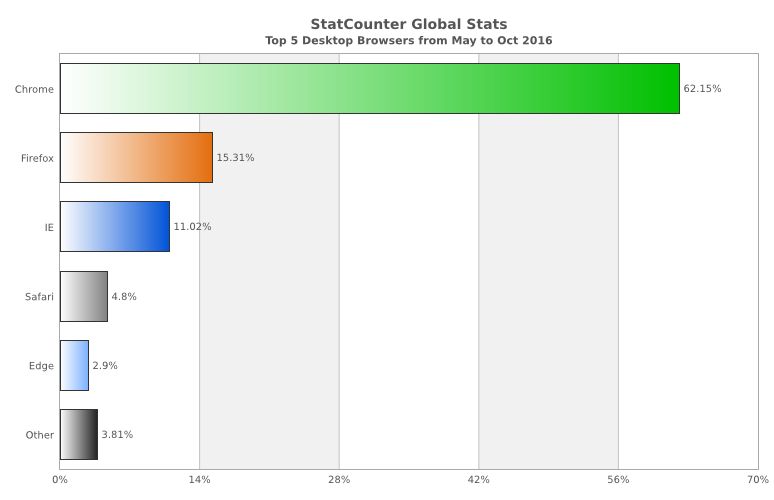
\includegraphics[scale=0.55]{StatCounter_browser_201605_201610_bar.png}
	\end{center}
\caption[Popolarità dei web browsers mag 2016 - ott 2016]{Popolarità dei web browser mag 2016 - ott 2016 \footnotemark}
\end{figure}
\footnotetext{\url{http://gs.statcounter.com/\#desktop-browser-ww-monthly-201605-201610-bar}} 

\section{Google Chrome}

Lanciato nel 2008 da parte di Google sulla base del progetto open source \textbf{Chromium}, il browser Google Chrome risulta esserne la versione compilata e distribuita da Google.
Al suo rilascio, nel settembre 2008, è stato reso pubblico anche il codice sorgente alla base di Chromium, con lo scopo di utilizzarlo come \textit{core} open source dell'applicazione, sottoponendolo nel frattempo alla revisione del codice da parte della comunità \footnote{\url{http://www.google.com/intl/it/chrome/timemachine/}}. 
Rispetto a Chromium, il cui sviluppo ed i suoi rilasci sono gestiti dalla comunità di sviluppatori, Google Chrome viene distribuito ed aggiornato da Google stessa secondo una propria tabella di marcia.
Le differenze fra i due browser si notano principalmente nella natura \textit{open source} o \textit{closed source}, con Google Chrome che annovera anche estensioni e plugin closed source al contrario di Chromium. \footnote{\url{https://chromium.googlesource.com/chromium/src/+/master/docs/chromium_browser_vs_google_chrome.md}} \nocite{Chromium}

La struttura e gestione della memoria cache risulta essere uguale fra i due browser.

\subsection{Struttura della memoria cache}

I file componenti la cache sono mantenuti in una cartella sul disco la cui locazione di default dipende dal sistema operativo in uso. Per sistemi Windows si ha: 

\begin{itemize}
	\item{\texttt{C:\textbackslash Users\textbackslash\%Username\%\textbackslash AppData\textbackslash Local\textbackslash Google\textbackslash Chrome\textbackslash User Data\textbackslash Default\textbackslash Cache}}
\end{itemize}

Nella cartella della cache sono presenti almeno 5 files: un file \textbf{\textit{index}} e 4 \textbf{\textit{data\_\# \footnote{Il \# indica un numero progressivo a partire da 0}}}. Altri file opzionali, detti \textbf{\textit{separate file}}, contengono informazioni la cui dimensione è maggiore di quella massima consentita per i file data\_\#.

\begin{figure}[h]
	\centering
	\begin{minipage}[c]{0.7\textwidth}
		\dirtree{%
			.1 \textit{\textbf{GOOGLE CHROME CACHE FOLDER}}.
			.2 \textit{Index file} \DTcomment{//Sempre presente}.
			.2 \textit{Block file data\_0} \DTcomment{//Sempre presente}.
			.2 \textit{Block file data\_1} \DTcomment{//Sempre presente}.
			.2 \textit{Block file data\_2} \DTcomment{//Sempre presente}.
			.2 \textit{Block file data\_3} \DTcomment{//Sempre presente}.
			.2 \textit{Separate file f\_\#\#\#\#\#\#}  \DTcomment{//Opzionale}.
			.2 \vdots.
			.2 \vdots.
			.2 \vdots.
			.2 \textit{Separate file f\_\#\#\#\#\#\#} \DTcomment{//Opzionale}.
		} 
	\end{minipage}
	\caption{Chrome: struttura della cartella \textit{cache}}
\end{figure}

\subsection{Struttura dei file}
Il file \textbf{\textit{index}} si presenta come una struttura formata da un \textit{index header} e da una \textit{tabella hash}. Il numero di elementi presenti nella tabella è definito dal parametro \textit{table\_len} presente nell'header. 

Qui gli elementi sono rappresentati secondo il formato \textbf{\textit{little endian}}. Ognuno di essi esprime il nome della risorsa (\textbf{\textit{key}}) e l'indirizzo in cache che la contiene. Convertendo in formato binario a 32 bit ed analizzandone le varie sezioni si ottiene la locazione esatta (file e posizione al suo interno) di una risorsa che presenta lo stesso \textit{hash}.

\begin{savenotes}
	\begin{table}[H]
		\rowcolors{2}{lightgray}{white}
		\begin{center}
			\resizebox{0.65\textwidth}{!}{
			\begin{tabular}{ccc}
				\textbf{Offset} &\textbf{Size} &\textbf{Description}\\  \hline
				If file type is 0 (Separate file) & &\\
				0.0 &28 bits &File number \footnote{Valore di \# in f\_\#\#\#\#\#\#}\\
				Else \\
				0.0 &16 bits &Block number \\
				2.0 &8 bits &File number (or file selector) \footnote{Valore di \# in data\_\#}\\
				3.0 &2 bits &Block size \footnote{Numero di blocchi contigui: 0 rappresenta 1 blocco, 3 rappresenta 4 blocchi}  \\
				3.2 &2 bits &Reserved\\
				Common  & &\\
				3.4 &3 bits &File type\\
				3.7 &1 bits &Initialized flag\\			
			\end{tabular}}
		\end{center}
		\caption{Chrome: struttura di un indirizzo cache}
	\end{table}
\end{savenotes}

\begin{table}[H]
	\rowcolors{2}{lightgray}{white}
	\begin{center}
		\resizebox{0.85\textwidth}{!}{
			\begin{tabular}{ccccccc}
				&Init &File type &Reserved &Contiguous blocks &File number  &Block number \\ \hline
				Binary &1 &010 &00 &00 &0000 0001 &0000 0000 0000 0011 \\
				Integer &1 &2 &0 &0 &1 &3 
			\end{tabular}}
	\end{center}
	\caption{Chrome: esempio di un indirizzo cache}
\end{table}

Interpretando il campo \textit{file type} nell'indirizzo si ottiene il file contenente la risorsa.
	
\begin{table}[H]
	\rowcolors{2}{lightgray}{white}
	\begin{center}
		\resizebox{0.6\textwidth}{!}{
		\begin{tabular}{ccc}
			\textbf{Binary} &\textbf{Integer} &\textbf{Interpretation}\\  \hline
			000 & 0 &Separate file\\
			001 & 1 &Ranking (36 byte block file)\\
			010 & 2 &256 byte block file\\
			011 & 3 &1 KByte block file\\
			100 & 4 &4 KByte block file\\
		\end{tabular}}
	\end{center}
	\caption{Chrome: tipi di file presenti nella cache}
\end{table}


I data\_\# file, indicati anche come \textbf{\textit{block file}}, sono costituiti da un \textit{header} seguito da un numero variabile (con un massimo di 64000) di \textit{blocchi} aventi dimensione fissa. Se venisse richiesta la presenza di ulteriori blocchi della stessa dimensione, un nuovo file data\_\# viene creato e collegato al precedente mediante il campo \textit{next\_file} presente nell'header. 
All'interno dei block file le informazioni vengono memorizzate utilizzando un massimo di 4 blocchi consecutivi. Se la dimensione dell'informazione da memorizzare dovesse superare quella di 4 blocchi consecutivi, questa viene memorizzata in un data file\_\# con blocchi di dimensioni maggiori. Se nessun data\_\# file è in grado di poter contenere l'informazione, questa viene salvata all'interno di \textbf{\textit{separate file}}
\newline

I \textbf{\textit{separate file}} (\textit{f\_\#\#\#\#\#\#}) memorizzano le informazioni di dimensioni maggiori di 16 KByte. 
Il loro nome è espresso nella forma \textit{f\_} seguito da un numero esadecimale progressivo di 6 cifre. 
Questo tipo di file non presenta header ma contiene solamente dati.
\newline

Sia le risorse di dimensioni fino a 16 KByte nei \textit{data\_\# file}, sia quelle di dimensioni maggiori che risiedono nei \textit{f\_\#\#\#\#\#\#}, sono memorizzate in formato \textbf{\textit{gzip}}. 
\clearpage

\begin{figure}[htpb]
	\begin{center}
		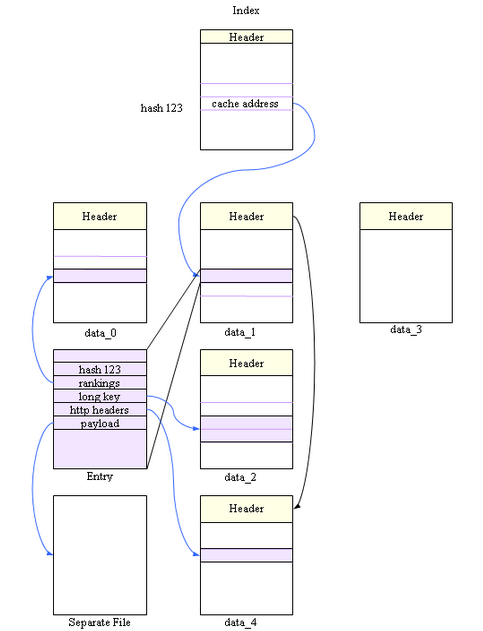
\includegraphics[scale=0.8]{Chrome_cache_overview.png}
	\end{center}
	\caption[Chrome: diagramma della cache]{Chrome: diagramma della cache \footnotemark}
\end{figure}
\footnotetext{\url{https://www.chromium.org/developers/design-documents/network-stack/disk-cache}}

Questo tipo di implementazione della memoria cache è valido per le versioni 1 e 2. Attualmente è in corso di sviluppo una nuova versione (v3) che renderà valido il modello di cache appena descritto solo per file salvati nelle versioni 1 e 2 \footnote{\url{https://www.chromium.org/developers/design-documents/network-stack/disk-cache/disk-cache-v3}}.
\clearpage

\section{Mozilla Firefox}

La fondazione Mozilla è un'organizzazione senza scopo di lucro con la missione di promuovere un Internet ``aperto ed accessibile a tutti''. \footnote{\url{https://www.mozilla.org/it/mission/}} 
Per questo sviluppa e rilascia \textbf{\textit{Firefox}}, un browser che propone fra le sue caratteristiche principali quella della sicurezza e della privacy durante la navigazione. \footnote{\url{https://www.mozilla.org/it/firefox/desktop/}}

Il progetto Mozilla fu lanciato il 31 Marzo 1998 con il rilascio in versione gratuita del codice sorgente del browser ``Netscape'' \footnote{\url{https://www.mozilla.org/en-US/about/history/details/}}. Supportato e sviluppato da una comunità indipendente, ne viene considerato il suo successore. Dal suo primo rilascio nel 2004 si è rivelato uno dei browser più apprezzati, rimanendo tuttora stabilmente tra quelli più utilizzati. 

\subsection{Struttura della memoria cache}

A partire dalla versione 32 del browser Firefox(settembre 2014 \footnote{\url{https://www.mozilla.org/en-US/firefox/32.0/releasenotes/}}), Mozilla ha introdotto un nuovo formato di cache per il proprio browser. \`E possibile trovare la directory contenente la cache alla locazione (per sistemi Windows):

\begin{itemize}
	\item{\texttt{C:\textbackslash Users\textbackslash\%Username\%\textbackslash AppData\textbackslash Local\textbackslash Mozilla\textbackslash Firefox\textbackslash Profiles\\\textbackslash random \footnote{Sequenza di 8 caratteri alfanumerici causali}.default\textbackslash Cache}}
\end{itemize}

All'interno di questa locazione si trovano varie sottocartelle in uso dal browser, compresa la cartella \textbf{\textit{cache2}} che contiene i file interessati. Scorrendo gli elementi presenti si trova un file \textbf{\textit{index}} al cui interno sono presenti record per ogni file presente nella cache. Le risorse vere e proprie, puntate dai record del file index si trovano in una sottocartella \textbf{\textit{entries}}.

\begin{figure}[h]
	\centering
	\begin{minipage}[c]{0.7\textwidth}
		\dirtree{%
			.1 \textit{\textbf{MOZILLA FIREFOX CACHE2 FOLDER}}.
			.2 \textit{Index File}.
			.2 \textit{Index.log File}.
			.2 \textit{Doomed folder}.
			.2 \textit{Entries folder}.
			.3 \textit{Entry}.
			.3 \vdots.
			.3 \vdots.
			.3 \vdots.
			.3 \textit{Entry}.
	} 
	\end{minipage}
	\caption{Firefox: struttura della cartella \textit{cache2}}
\end{figure}

\subsection{Struttura dei file}

Il file \textbf{\textit{index}} si presenta come una struttura formata da un \textit{header} e da una \textit{tabella hash} contenente i record che puntano alle \textit{entries} nella cartella \textbf{\textit{entries}}. \nocite{Habben}

I record nella tabella hash sono rappresentati secondo il formato \textbf{\textit{big endian}} ed indicano una risorsa contenuta all'interno di uno dei file nella cartella entries. 
\clearpage

Ogni record ha dimensione di 36 byte ed è così formato:


\begin{table}[H]
	\rowcolors{2}{lightgray}{white}
	\begin{center}
		\resizebox{0.7\textwidth}{!}{
			\begin{tabular}{cccc}
				\textbf{Offset} &\textbf{Size} &\textbf{Type} &\textbf{Description}\\  \hline
				0 &20 &SHA1 &Hash Of URL\\
				20 &4 &BE integer &Frequency\\
				24 &4 &BE Unix date &Expiration date\\
				28 &4 &BE integer &AppId \\
				32 &1 &Byte &Flags\\
				33 &3 &BE integer &File size \\
			\end{tabular}}
		\end{center}
		\caption{Firefox: struttura di un indirizzo cache}
\end{table}

\begin{table}[H]
	\begin{center}
		\resizebox{0.9\textwidth}{!}{
			\begin{tabular}{cccccc}
				Hash &Frequency &Exp date (Unix) &AppId &Flags  &File size \\ \hline
				2BD1F3E105AFF6A7CBFB &1025038823 &1481233511 &0 &128 &99 \\
				14955D5FA38873035CB5
			\end{tabular}}
		\end{center}
		\caption{Firefox: esempio di un indirizzo cache}
	\end{table}

I primi 20 byte rappresentano l'hash SHA1 dell'url della risorsa ed è con questo che vengono nominati i file all'interno della cartella \textit{entries}.

Questi file non presentano header ed il loro contenuto, rappresentato in formato \textbf{\textit{big endian}}, comincia a partire dalla prima locazione.
Alla fine del contenuto si trovano i metadati provenienti dal server web, come ad esempio l'header HTTP. Per conoscerne l'esatta posizione bisogna leggere gli ultimi 4 byte del file.
A partire dalla locazione indicata da questi si trovano in ordine 4 byte rappresentanti l'hash del contenuto del file, seguiti da porzioni di 2 byte dell'hash per ogni blocco da 256 KByte in cui può essere diviso il file.  
Dividendo la dimensione del file (in byte) per la dimensione del blocco (in byte) e arrotondando per eccesso in caso di resto della divisione, si ottiene il numero di blocchi presenti all'interno del file,  
A questo punto si moltiplica il numero di blocchi trovato per 2 (porzione di hash contenuta in ogni blocco), si aggiungono i 4 byte dell'hash del contenuto del file e si ottiene l'offset esatto di partenza per i metadati.

\begin{savenotes}
	\begin{table}[H]
		\rowcolors{2}{lightgray}{white}
		\begin{center}
			\resizebox{0.7\textwidth}{!}{
				\begin{tabular}{cccc}
					\textbf{Offset} &\textbf{Size} &\textbf{Type} &\textbf{Description}\\  \hline
					0 &4 &BE integer &Version\\
					4 &4 &BE integer &Fetch count\\
					8 &4 &BE Unix date &Last Fetched date\\
					12 &4 &BE Unix date &Last Modified Date \\
					16 &4 &BE integer &Frecency \footnote{\url{https://developer.mozilla.org/en-US/docs/Mozilla/Tech/Places/Frecency_algorithm}}\\
					20 &4 &BE Unix date &Expiration date \\
					24 &4 &BE Unix date &Key lenght\\
					28 &[Key lenght] &String &URI
				\end{tabular}}
			\end{center}
			\caption{Firefox: struttura di un record in un \textit{entry file}}
	\end{table}
\end{savenotes}

\clearpage

\section{Opera}

Sviluppato dall'azienda \textit{Opera Software} a partire dal 1996, si è distinto per l'inserimento di importanti funzioni adottate successivamente anche da altri browser, come il supporto ai fogli di stile \textit{CSS} \footnote{\url{http://meyerweb.com/eric/articles/webrev/199906.html}} o la possibilità di cancellare i dati della navigazione . \footnote{\url{http://www.slashgeek.net/2012/06/08/5-features-opera-browser-did-first/}}

Il rilascio della versione 15 segna l'abbandono al motore di rendering \textit{Presto} in favore di \textit{Blink} (fork del \textit{WebKit rendering engine}) ma soprattutto introduce importanti modifiche al codice sorgente del browser. 

A partire da questa versione infatti, il codice sorgente è basato sul codice del browser Chromium \footnote{\url{http://www.opera.com/docs/changelogs/unified/1500/}}, permettendo ad Opera, per quanto riguarda la memoria cache, di avere la stessa struttura e di comportarsi esattamente come i browser Chrome e Chromium.


			
			% stile pagina vuoto. Inizia nuovo capitolo su pagina destra per documenti doppia facciata. Rimuove header da eventuale pagina bianca lasciata
			\clearpage{\pagestyle{empty}\cleardoublepage}
			
			\chapter{Browser Cache Analyzer}

\textit{Browser Cache Analyzer} è l'applicazione che è stata sviluppata per eseguire l'analisi della memoria cache dei browser presi in esame.

Permette di ottenere un'anteprima del contenuto lasciando decidere all'utente se effettuarne una successiva estrazione, creando una copia dei dati presenti in memoria cache e fornendo un report finale in formato Html per consentire una più facile consultazione dei risultati.

Progettata per sistemi Windows, presenta un'architettura divisa in \textit{moduli}. Questo la rende flessibile, permettendo di aggiungere nuove funzionalità, come ad esempio il supporto ad altri browser.

\subsection{Implementazione: linguaggi e librerie utilizzate}
Il corpo principale dell'applicazione è stato scritto con il linguaggio di programmazione \textbf{\textit{Python}} mentre la creazione e la gestione dell'interfaccia grafica è affidata al framework \textbf{\textit{Qt}}. Ci si è avvalso anche dell'utilizzo di librerie di terze parti come \textbf{\textit{Psutil}} per informazioni sui processi in uso dal sistema operativo o del programma \textbf{\textit{PyInstaller}} per la creazione del file eseguibile.

\clearpage
\subsubsection{Python}
\nocite{Python}
Alla fine degli anni 80, l'olandese Guido van Rossum iniziò a sviluppare un linguaggio di programmazione che facesse della semplicità uno dei suoi maggiori punti di forza: il \textbf{\textit{Pyhton}}. 

Python è un linguaggio multi-piattaforma ed orientato agli oggetti che supporta caratteristiche quali il \textit{dynamic typing}, che evita errori di tipo sui valori delle varie operazioni, o la \textit{name resolution}, che determina a quale identificatore riferirsi in uno specifico contesto, permettendo così di associare lo stesso nome anche ad oggetti differenti durante l'esecuzione del programma. I blocchi di istruzione all'interno dell'applicazione vengono delimitati dall'intentazione e non da parentesi, garantendo così un'alta leggibilità del codice. Pyhton prevede che la gestione della memoria sia a carico di un \textit{garbage-collector}.

Come tutti i linguaggi interpretati, le sue prestazioni non possono essere comparate a quelle dei linguaggi compilati, specie per applicazioni che richiedono un elevato carico computazionale, ma risultano in linea o superiori a quelle degli altri linguaggi interpretati.

Anche grazie alla sua filosofia, cioè quella di un linguaggio che presenta un elevato numero di librerie standard e al contempo di essere altamente estensibile, è possibile introdurre tutti i moduli per le funzionalità richieste. 
\'E anche possibile scrivere ed integrare estensioni C / C++, potendo così sfruttare le elevate prestazioni di un linguaggio compilato ove richiesto, continuando a beneficiare nel contempo della versatilità del Python.  

\subsubsection{Qt e PyQt} 
\nocite{Qt}
\nocite{PyQt}
Lo sviluppo di \textbf{\textit{Qt}} è iniziato nel 1990 da parte di Eirik Chambe-Eng and Haavard Nord della compagnia norvegese Trolltech. Qt è un framework multi-piattaforma per lo sviluppo di applicazioni in ambiente desktop, embedded e mobile. Scritto in C++, grazie al preprocessore \textit{MOC} (Meta-Object Compiler) ne estende le funzionalità.
Prima della compilazione, il MOC effettua un parsing del codice sorgente in Qt-extended C++ generando un codice conforme al C++. 

Fra le caratteristiche aggiunte, la principale è quella riguardante i \textit{segnali e slot}, utilizzati per la comunicazione fra i vari oggetti dell'applicazione. 

\begin{figure}[htpb]
	\begin{center}
		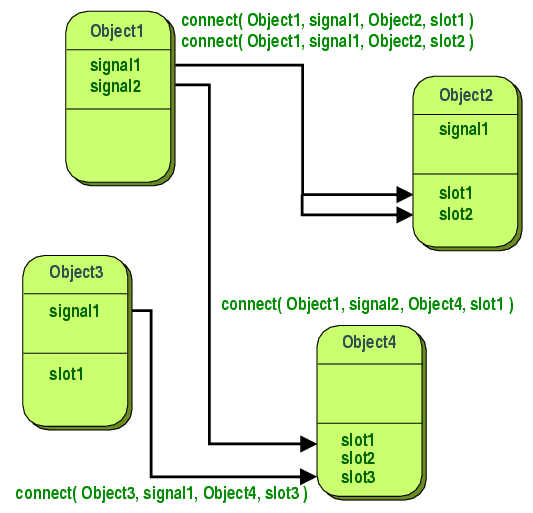
\includegraphics[scale=0.5]{Signal_slot_view.png}
	\end{center}
	\caption[Segnali e slot]{Segnali e slot \footnotemark}
\end{figure}
\footnotetext{\url{http://doc.qt.io/qt-5/signalsandslots.html}}


Al verificarsi di un evento, ad esempio la pressione di un tasto, viene emesso un segnale. Il segnale viene intercettato da uno slot, cioè una funzione con il compito di gestirlo. 
Segnali e slot sono collegati in maniera \textit{loosely coupled}, cioè la classe che emette il segnale non ha conoscenza dello slot che andrà a ricevere il segnale. Sarà il meccanismo Qt che si occupa di gestire i segnali e gli slot a far si che il giusto slot venga richiamato, con i giusti parametri, alla ricezione del segnale. I segnali sono \textit{type safe}, ovvero la signature di un segnale deve combaciare con quella dello slot ricevente. Un segnale è una funzione pubblica e può essere emesso ovunque all'interno dell'applicazione, anche se vi è la raccomandazione di emetterlo dalla classe che lo ha generato o dalle sue sottoclassi.

Così come le classi che emettono il segnale, anche le funzioni che li ricevono non hanno conoscenza dei segnali ai quali sono collegate. Possono essere usate sia per connettere segnali provenienti dai vari oggetti oppure essere utilizzate come normali funzioni, garantendo in questo modo che i componenti siano tra loro indipendenti. Lo slot viene eseguito immediatamente alla ricezione del segnale in modo totalmente indipendente dall'esecuzione della GUI mentre il codice successivo all'istruzione \textit{emit} nella classe che ha emesso il segnale, sarà eseguito non appena lo slot avrà eseguito il \textit{return} tranne in caso di \textit{queued connections} in cui sarà lo slot ad essere eseguito successivamente al codice seguente l'istruzione \textit{emit}.

I segnali, che non possono effettuare il return essendo di tipo \textit{void}, vengono generati dal MOC e non vengono implementati nel file sorgente. 

Per poter utilizzare il framework Qt con Python è stato necessario utilizzare \textbf{\textit{PyQt}}. PyQt permette di effettuare un \textit{binding}, cioè un collegamento, tra il Python e il framework Qt. Questi collegamenti sono implementati tramite moduli Python contenenti più di 1000 classi.

Sviluppato dalla \textit{Riverbank}, il framework PyQt include astrazioni per una moltitudine di oggetti quali il meccanismo per la gestione degli slot e dei segnali, network sockets, threads, Unicode, regular expressions, SQL databases, SVG, OpenGL ed altri ancora. Possiede
anche un web browser pienamente funzionante ed un insieme di GUI widgets.

Un altro componente importante presente in PyQt è il \textbf{\textit{Qt Designer}}, strumento che permette la creazione di interfacce grafiche. 
Le interfacce vengono create disponendo gli oggetti su quella che diventerà una finestra dell'applicazione, facilitando la disposizione degli stessi in layout, permettendo di settarne le proprietà e consentendo anche la creazione delle connessioni fra segnali e slot dei vari oggetti.

\clearpage

\begin{figure}[htpb]
	\begin{center}
		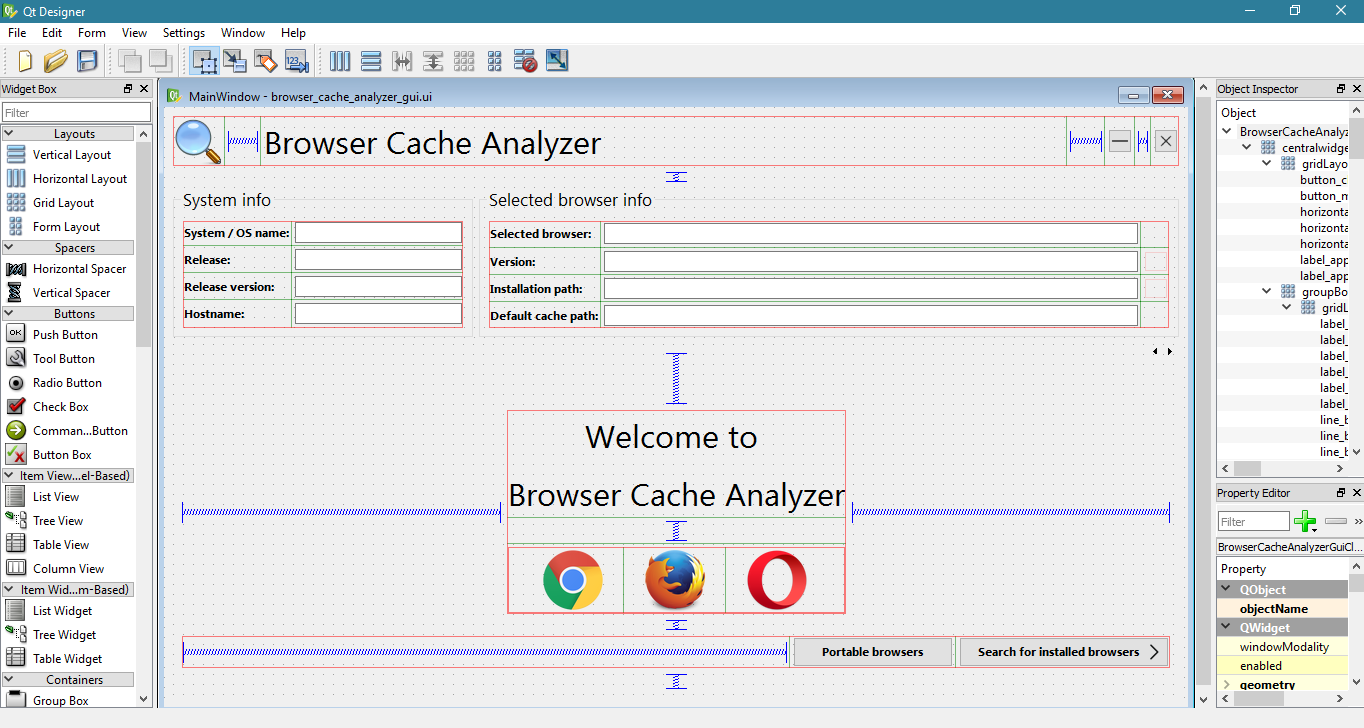
\includegraphics[scale=0.42]{Welcome_screen_designer.png}
	\end{center}
	\caption[Schermata di benvenuto dell'applicazione in QtDesigner]{Schermata di benvenuto dell'applicazione in QtDesigner}
\end{figure}

PyQt inoltre presenta anche un insieme di \textit{utilities} quali:

\begin{itemize}
	\item{pyuic4: corrisponde all'utility \textit{uic} di Qt. Converte le GUI create con QtDesigner in codice Python}
	\item{pyrcc4: corrisponde all'utility \textit{rcc} di Qt. Incorpora risorse esterne (ad esempio icone ed immagini) descritte in un file all'interno di un modulo Python }
\end{itemize} 

\clearpage

\subsubsection{Psutil}
\textbf{\textit{Psutil}} \footnote{\url{https://pypi.python.org/pypi/psutil}} è una libreria multi-piattaforma per Python. Fornisce \textit{utilities} per ottenere informazioni sui processi in esecuzione nel sistema ed utilizzo delle varie risorse (memoria, disco, rete). Implementa anche funzionalità e comandi offerti dalla \textit{command line} come ps, top, lsof, netstat, ifconfig, who, df, kill, free ed altre.

\subsubsection{PyInstaller}
\textbf{\textit{PyInstaller}} \footnote{\url{http://www.pyinstaller.org/}} è un programma che permette la creazione di eseguibili \textit{stand alone} a partire da sorgenti Python. Multi-piattaforma, utilizza il supporto del supporto del sistema operativo per il caricamento di librerie dinamiche, assicurando così piena compatibilità con \textit{packages} di terze parti come PyQt.
\clearpage

\subsection{Descrizione delle componenti}
Di seguito viene fornita una visione della struttura completa dell'applicazione e ne verranno illustrati i vari moduli che la compongono.

\begin{figure}[htpb]
	\begin{center}
		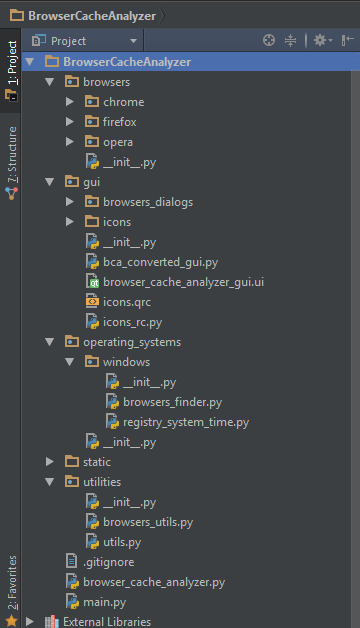
\includegraphics[scale=0.8]{Struttura_applicazione.png}
	\end{center}
	\caption[Struttura dell'applicazione Browser Cache Analyzer]{Struttura dell'applicazione Browser Cache Analyzer}
\end{figure}

\subsubsection{Modulo Browser}
Il modulo \textbf{\textit{Browsers}} è il modulo contenente la logica e le funzioni che permettono di eseguire l'analisi e l'esportazione del contenuto della memoria cache. 
Al suo interno sono contenuti altri moduli, uno per ogni browser preso in esame. 
La scelta di creare il modulo \textit{browsers} è stata presa per poter separare la logica di funzionamento dell'applicazione da quella dei browser. In questo modo aggiungere un nuovo browser o modificare il comportamento di uno già presente, ad esempio a seguito di modifiche o nuove implementazioni della memoria cache da parte del produttore, comporta solo minime modifiche al codice dell'applicazione, volte solo all'aggiunta delle nuove funzionalità.

\begin{figure}[htpb]
	\begin{center}
		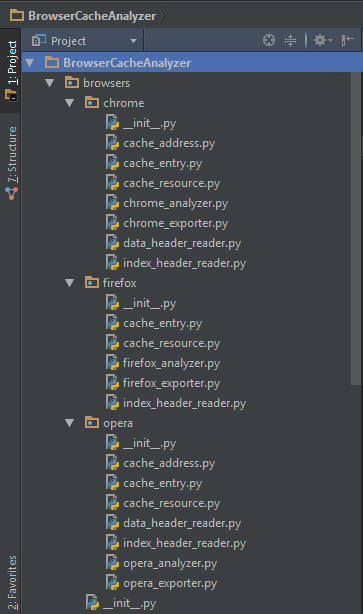
\includegraphics[scale=0.6]{Modulo_browsers.png}
	\end{center}
	\caption[Browser Cache Analyzer: modulo \textbf{\textit{browsers}}]{Browser Cache Analyzer: modulo \textbf{\textit{browsers}}}
\end{figure}

%Si possono osservare i vari file che al loro interno presentano classi e funzioni che ricalcano gli oggetti presenti in memoria cache. Ad %esempio le funzioni \textit{read_index_header}  


			
			
% ********************************************************************
% Materiale finale
%******************************************************************

	% stile pagina vuoto. Inizia nuovo capitolo su pagina destra per documenti doppia facciata. Rimuove header da eventuale pagina bianca lasciata
	\clearpage{\pagestyle{empty}\cleardoublepage}
	
	% riferimento ipertestuale per "Elenco figure"
	\phantomsection \label{listoffigures}
	
	% aggiungere voce "Elenco figure" nell'indice
	\addcontentsline{toc}{chapter}{Elenco delle figure}
	
	% stile pagina vuoto (no header e no footer)
	\pagestyle{empty}
	
	% creazione elenco figure
	\listoffigures 	
	
	% stile pagina vuoto. Inizia nuovo capitolo su pagina destra per documenti doppia facciata. Rimuove header da eventuale pagina bianca lasciata
	\clearpage{\pagestyle{empty}\cleardoublepage}
	
	% riferimento ipertestuale per "Elenco tabelle"
	\phantomsection \label{listoftables}
	
	% aggiungere voce "Elenco tabelle" nell'indice
	\addcontentsline{toc}{chapter}{Elenco delle tabelle}
	
	% stile pagina vuoto (no header e no footer)
	\pagestyle{empty}
	
	% creazione elenco tabelle
	\listoftables
	
	% stile pagina vuoto. Inizia nuovo capitolo su pagina destra per documenti doppia facciata. Rimuove header da eventuale pagina bianca lasciata
	\clearpage{\pagestyle{empty}\cleardoublepage}
	
	% cambiare nome bibliografia
	\renewcommand{\bibname}{Riferimenti}
	
	% riferimento ipertestuale per "Bibliografia"
	\phantomsection \label{Riferimenti}
	
	% aggiungere voce "Bibliografia" nell'indice
	\addcontentsline{toc}{chapter}{Riferimenti}
	
	% Opere contrassegnate da etichette formate a partire da nome autore e anno pubblicazione (bab = lingua del documento)
	\bibliographystyle{babalpha}
	
	% stile pagina vuoto (no header e footer)
	\pagestyle{empty}
	
	% creazione bibliografia e percorso (relativo) file bibliografia 
	\bibliography{./Riferimenti/Riferimenti}

\end{document}
